\begin{problem}{Cross-Stitch}{standard input}{standard output}{2 seconds}{512 megabytes}

Cross-stitch is a form of needlework known since prehistoric times. A cross-stitch pattern consists of several crosses on the face of the fabric, that are connected on the backside. Traditionally, the whole pattern should be embroidered by one thread.

Carol is going to mass-produce cross-stitch patterns. Each pattern will be accompanied by the rectangular patch of fabric and the thread that is required to embroider this pattern. Carol wants to minimize the length of the thread that is required for the pattern.\\
\centerline{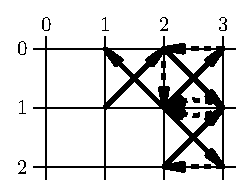
\includegraphics{cross-stitch-1.ps}}\\
You are given the face of the pattern. You should design the backside, so that the total length of the thread is minimal. The crosses on the pattern's face are 8-connected, i.e. it is possible to reach each cross from any other by a sequence of chess king's moves.

\InputFile
The first line of the input contains two integers $w$ and $h$~--- the width and the height of the patch of fabric ($1 \le w, h \le 100$).

The following $h$ lines contain the face of the pattern. Each of them contains $w$ characters, where `\texttt{X}' represents a cross, and `\texttt{.}'~--- an empty space. The face of the pattern contains at least one cross and crosses are 8-connected.

\OutputFile
The first line of output should contain the single integer $n$~--- the number of stitches required to embroider the pattern. 

The following $n + 1$ lines should contain the coordinates of the points where a needle comes from the backside to the face or back: $x_i$, $y_i$ for $i=0..n$. The upper-left corner of the patch has coordinates $(0, 0)$, and the bottom-right one~--- $(w, h)$. The first stitch goes to the face of the pattern, the second one~--- to the backside, the third one~--- to the face, and so on. It is possible to duplicate stitches at the backside, but not at the face. None of the stitches should have zero length.

\Example

\begin{example}
\exmpfile{example.01}{example.01.a}%
\end{example}

\end{problem}

